\subsection{Voltage Divider Bias Circuit:}

For the following experiment we assemble the circuit in Figure 3.2.0. The procedure consist in exchange between two {\bfseries\itshape NPN} transistors ( {\bfseries\itshape 2N2222A} and {\bfseries\itshape BC547C} ) and compare in Table 2 the measured values. \hfill \break

Once we had the circuit, we proceed to measure $V_{B}$, $V_{C}$, $V_{CE}$, $I_{B}$, $I_{C}$, $I_{E}$: \hfill \break

\begin{multicols}{2}
\begin{figure}[H]
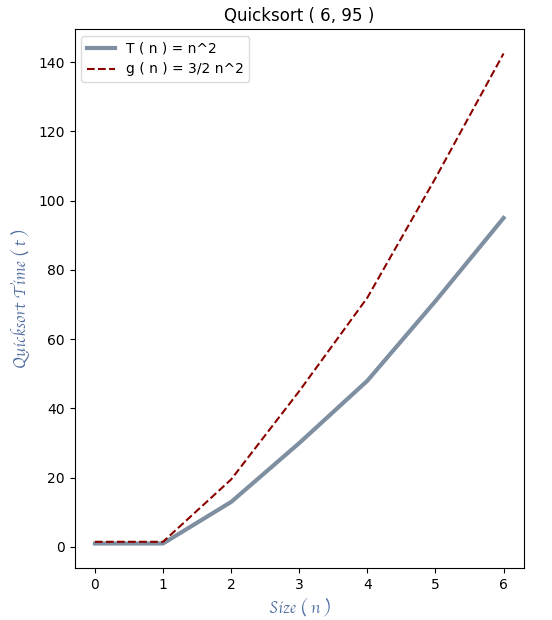
\includegraphics[scale=1.4]{p1.png}
\centering \linebreak \linebreak Figure 3.2.0: Voltage divider bias circuit using a 2N2222A transistor.
\end{figure}

\begin{tasks}
\task For $V_{B}$: The Base Voltage can be measured by connecting the positive terminal of the voltmeter on the {\bfseries\itshape Base} terminal of the transistor, and the negative terminal of the voltmeter on the {\bfseries\itshape Ground} reference.
\task For $V_{C}$: The Collector Voltage can be measured by connecting the positive terminal of the voltmeter on the {\bfseries\itshape Collector} terminal of the transistor, and the negative terminal of the voltmeter on the {\bfseries\itshape Ground} reference.
\task For $V_{CE}$: The Emitter-Collector Voltage can be measured by connecting the positive terminal of the voltmeter on the {\bfseries\itshape Collector} terminal, and the negative terminal of the voltmeter on the {\bfseries\itshape Emitter} terminal.
\task For $I_{B}$: The Base current can be measured by connecting the ammeter in series with the node that connects {\bfseries\itshape $R_{1}$} and {\bfseries\itshape $R_{2}$} and the {\bfseries\itshape Base} terminal of the transistor.
\task For $I_{C}$: The Collector current can be measured by connecting the ammeter in series with {\bfseries\itshape $R_{C}$} and the {\bfseries\itshape Collector} terminal of the transistor.
\task For $I_{E}$: The Emitter current can be measured by connecting the ammeter in series with {\bfseries\itshape $R_{E}$} and the {\bfseries\itshape Emitter} terminal of the transistor.
\end{tasks}
\end{multicols} \hfill

{\bfseries\itshape\color{carmine}{Observation:}} {\itshape\color{carmine}{The procedure for measuring this values using the {\bfseries BC547C} or the {\bfseries 2N2222A} transistors it's relative the same.}} \hfill \break

\begin{center}
\begin{tabular}[1.5cm]{c c c}
\toprule
\toprule
\centering \hspace{120pt} & \hspace{50pt} {\bfseries 2N2222A} \hspace{50pt}  & \hspace{50pt} {\bfseries BC547C} \hspace{50pt} \\
\midrule
\midrule
$V_{B}$ & 2.38 V & 2.46 V \\
\cmidrule{1-3}
$V_{C}$ & 7.6 V & 7.4 V \\
\cmidrule{1-3}
$V_{CE}$ & 5.8 V & 5.6 V \\
\cmidrule{1-3}
$I_{B}$ & 2 $\mu$A & 2 $\mu$A \\
\cmidrule{1-3}
$I_{C}$ & 7.6 mA & 8.2 mA \\
\cmidrule{1-3}
$I_{E}$ & 7.9 mA & 8.2 mA \\
\bottomrule
\linebreak
\end{tabular}
\linebreak Table 2: Measured values for Figure 3.2.0.
\end{center}

\pagebreak